\scanpage{53}
% E: text|printed header, upper left|//* CRAY2 0411 I
\texttt{//*\quad CRAY2\quad 0411\qquad I}

% E: drawing|printed upper banner|four zero characters formed from zeros
\figure{
\begin{tikzpicture}[x=.09cm,y=.14cm,every node/.style={font=\tiny\ttfamily,anchor=west,inner sep=0pt}]
\foreach \d in {0,14,28,42}{
\node at ({\d+11},0) {00000000};
\node at ({\d+9},-1) {0000000000};
\node at ({\d+7},-2) {00}; \node at ({\d+15},-2) {0000};
\node at ({\d+6},-3) {00}; \node at ({\d+13},-3) {00}; \node at ({\d+16},-3) {00};
\node at ({\d+5},-4) {00}; \node at ({\d+11},-4) {00}; \node at ({\d+15},-4) {00};
\node at ({\d+4},-5) {00}; \node at ({\d+9},-5) {00}; \node at ({\d+14},-5) {00};
\node at ({\d+3},-6) {00}; \node at ({\d+7},-6) {00}; \node at ({\d+13},-6) {00};
\node at ({\d+2},-7) {00}; \node at ({\d+5},-7) {00}; \node at ({\d+12},-7) {00};
\node at ({\d+1},-8) {0000}; \node at ({\d+11},-8) {00};
\node at (\d,-9) {000}; \node at ({\d+10},-9) {00};
\node at (\d,-10) {0000000000};
\node at (\d,-11) {00000000};
}
\end{tikzpicture}}

% E: drawing|printed middle banner|CRAY2 formed from repeated characters
\figure{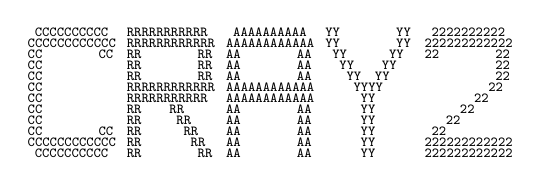
\begin{tikzpicture}[x=.09cm,y=.14cm,every node/.style={font=\tiny\ttfamily,anchor=west,inner sep=0pt}]
\node at (1,0) {CCCCCCCCCC}; \node at (0,-1) {CCCCCCCCCCCC};
\foreach \r in {2,3,4,5,6,7,8,9}{\node at (0,-\r) {CC};}
\node at (10,-2) {CC}; \node at (10,-9) {CC};
\node at (0,-10) {CCCCCCCCCCCC}; \node at (1,-11) {CCCCCCCCCC};
\node at (14,0) {RRRRRRRRRRR}; \node at (14,-1) {RRRRRRRRRRRR};
\foreach \r in {2,3,4,7,8,9,10,11}{\node at (14,-\r) {RR};}
\foreach \r in {2,3,4}{\node at (24,-\r) {RR};}
\node at (14,-5) {RRRRRRRRRRRR}; \node at (14,-6) {RRRRRRRRRRR};
\node at (20,-7) {RR}; \node at (21,-8) {RR}; \node at (22,-9) {RR}; \node at (23,-10) {RR}; \node at (24,-11) {RR};
\node at (29,0) {AAAAAAAAAA}; \node at (28,-1) {AAAAAAAAAAAA};
\foreach \r in {2,3,4,7,8,9,10,11}{\node at (28,-\r) {AA}; \node at (38,-\r) {AA};}
\node at (28,-5) {AAAAAAAAAAAA}; \node at (28,-6) {AAAAAAAAAAAA};
\foreach \r in {0,1}{\node at (42,-\r) {YY}; \node at (52,-\r) {YY};}
\node at (43,-2) {YY}; \node at (51,-2) {YY};
\node at (44,-3) {YY}; \node at (50,-3) {YY};
\node at (45,-4) {YY}; \node at (49,-4) {YY};
\node at (46,-5) {YYYY};
\foreach \r in {6,7,8,9,10,11}{\node at (47,-\r) {YY};}
\node at (57,0) {2222222222}; \node at (56,-1) {222222222222};
\node at (56,-2) {22}; \node at (66,-2) {22};
\node at (66,-3) {22}; \node at (66,-4) {22}; \node at (65,-5) {22}; \node at (63,-6) {22}; \node at (61,-7) {22}; \node at (59,-8) {22}; \node at (57,-9) {22};
\node at (56,-10) {222222222222}; \node at (56,-11) {222222222222};
\end{tikzpicture}}

% E: text|printed middle-lower, six repeated lines|START JOB 411 CRAY2
\texttt{****A\quad START\quad JOB\quad 411\quad CRAY2\qquad ROOM\qquad 4.18.41 PM 16 AUG 82\quad R6.PR1\quad SYS JES2\quad JOB 411\quad START\quad A****}\par
\texttt{****A\quad START\quad JOB\quad 411\quad CRAY2\qquad ROOM\qquad 4.18.41 PM 16 AUG 82\quad R6.PR1\quad SYS JES2\quad JOB 411\quad START\quad A****}\par
\texttt{****A\quad START\quad JOB\quad 411\quad CRAY2\qquad ROOM\qquad 4.18.41 PM 16 AUG 82\quad R6.PR1\quad SYS JES2\quad JOB 411\quad START\quad A****}\par
\texttt{****A\quad START\quad JOB\quad 411\quad CRAY2\qquad ROOM\qquad 4.18.41 PM 16 AUG 82\quad R6.PR1\quad SYS JES2\quad JOB 411\quad START\quad A****}\par
\texttt{****A\quad START\quad JOB\quad 411\quad CRAY2\qquad ROOM\qquad 4.18.41 PM 16 AUG 82\quad R6.PR1\quad SYS JES2\quad JOB 411\quad START\quad A****}\par
\texttt{****A\quad START\quad JOB\quad 411\quad CRAY2\qquad ROOM\qquad 4.18.41 PM 16 AUG 82\quad R6.PR1\quad SYS JES2\quad JOB 411\quad START\quad A****}

% E: text|printed lower left, notice header|DERNIERE MISE A JOUR
\texttt{DERNIERE MISE A JOUR DE JOURNAL : 11-08-82}\par
\texttt{ATTENTION ...........}

% E: text|printed lower left, notice 1|ARRET DE L'ORDINATEUR
\texttt{1. ARRET DE L'ORDINATEUR LE MARDI 17 AOUT DE 7 H A 8 H.}

% E: text|printed lower left, notice 2|UNE MODIFICATION SYSTEME
\texttt{1\qquad 2. UNE MODIFICATION SYSTEME NOUS CONTRAINDRA A DETRUIRE}\par
\texttt{1\qquad\phantom{2. }LE CONTENU DU DISQUE SPOOL LE MARDI 17 AOUT A 6 HEURES}\par
\texttt{1\qquad\phantom{2. }VEUILLEZ RECUPERER VOS SORTIES EN ATTENTE AVANT CETTE}\par
\texttt{1\qquad\phantom{2. }DATE. MERCI DE VOTRE COMPREHENSION.}

% E: text|printed lower left, notice 3|UN ARRET EXCEPTIONNEL
\texttt{1\qquad 3. UN ARRET EXCEPTIONNEL POUR PREPARER L'ARRIVEE DE NOUVELLES}\par
\texttt{1\qquad\phantom{3. }UNITES AURA LIEU DU VENDREDI 20 AOUT A 17H \unsure{30} AU LUNDI}\par
\texttt{1\qquad\phantom{3. }23 AOUT A 8H.}

% E: drawing|handwritten bottom left|red crossing green polygon black edges
% E: drawing|handwritten bottom right|red crossing green polygon dashed chord
% E: drawing|handwritten bottom centre|long red separating curve
\figure{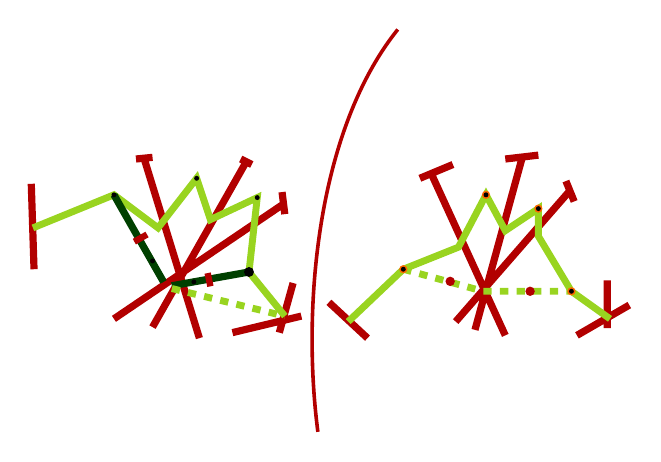
\begin{tikzpicture}[scale=.7]
\draw[red!70!black,line width=2.6pt] (0,2.8)--(.05,1.25) (2.05,3.25)--(3.05,0) (1.9,3.25)--(2.2,3.28) (2.2,.2)--(3.9,3.2) (3.8,3.25)--(4,3.15) (1.5,.35)--(4.6,2.45) (4.6,2.25)--(4.55,2.65) (3.65,.1)--(4.9,.4) (4.5,.1)--(4.75,1);
\draw[yellow!60!green,line width=2.5pt] (.03,2)--(1.5,2.6)--(2.3,2)--(3,2.9)--(3.25,2.15)--(4.1,2.55)--(3.95,1.2)--(4.6,.4);
\draw[green!25!black,line width=2.6pt] (1.5,2.6)--(2.4,1.02) (2.55,.95)--(3.95,1.2);
\draw[yellow!60!green,line width=2.5pt,dashed] (2.55,.9)--(4.6,.4);
\draw[red!70!black,line width=2.3pt] (1.87,1.75)--(2.1,1.88) (3.25,.94)--(3.2,1.18);
\foreach \p in {(1.5,2.6),(3,2.9),(4.1,2.55),(2.2,1.4),(2.95,1.02)}{\fill \p circle(.045);}
\fill (3.95,1.2) circle(.09);
\draw[red!70!black,line width=1.3pt] (6.65,5.6)..controls (5.2,3.8) and (4.9,.6)..(5.2,-1.7);
\begin{scope}[shift={(5.7,.2)}]
\draw[red!70!black,line width=2.6pt] (-.3,.45)--(.4,-.2) (1.55,2.8)--(2.9,-.15) (1.35,2.7)--(1.95,2.95) (2.35,-.05)--(3.2,3.05) (2.9,3.05)--(3.5,3.12) (2,.1)--(4.05,2.45) (4,2.65)--(4.15,2.28) (4.2,-.15)--(5.15,.4) (4.75,-.02)--(4.75,.85);
\draw[yellow!60!green,line width=2.5pt] (.05,.1)--(1.05,1.05)--(2.05,1.45)--(2.55,2.4)--(2.9,1.75)--(3.5,2.15)--(3.5,1.65)--(4.1,.65)--(4.8,.15);
\draw[yellow!60!green,line width=2.5pt,dashed] (1.05,1.05)--(2.5,.65)--(4.1,.65);
\foreach \p in {(1.05,1.05),(2.55,2.4),(3.5,2.15),(4.1,.65)}{\fill[orange!80!red] \p circle(.075); \fill \p circle(.045);}
\fill[red!70!black] (1.9,.83) circle(.085) (3.35,.65) circle(.085);
\end{scope}
\end{tikzpicture}}
\mspage{52}
